% FIXED!

\newcommand{\figModel}{
\begin{figure}[t]
    \centering
    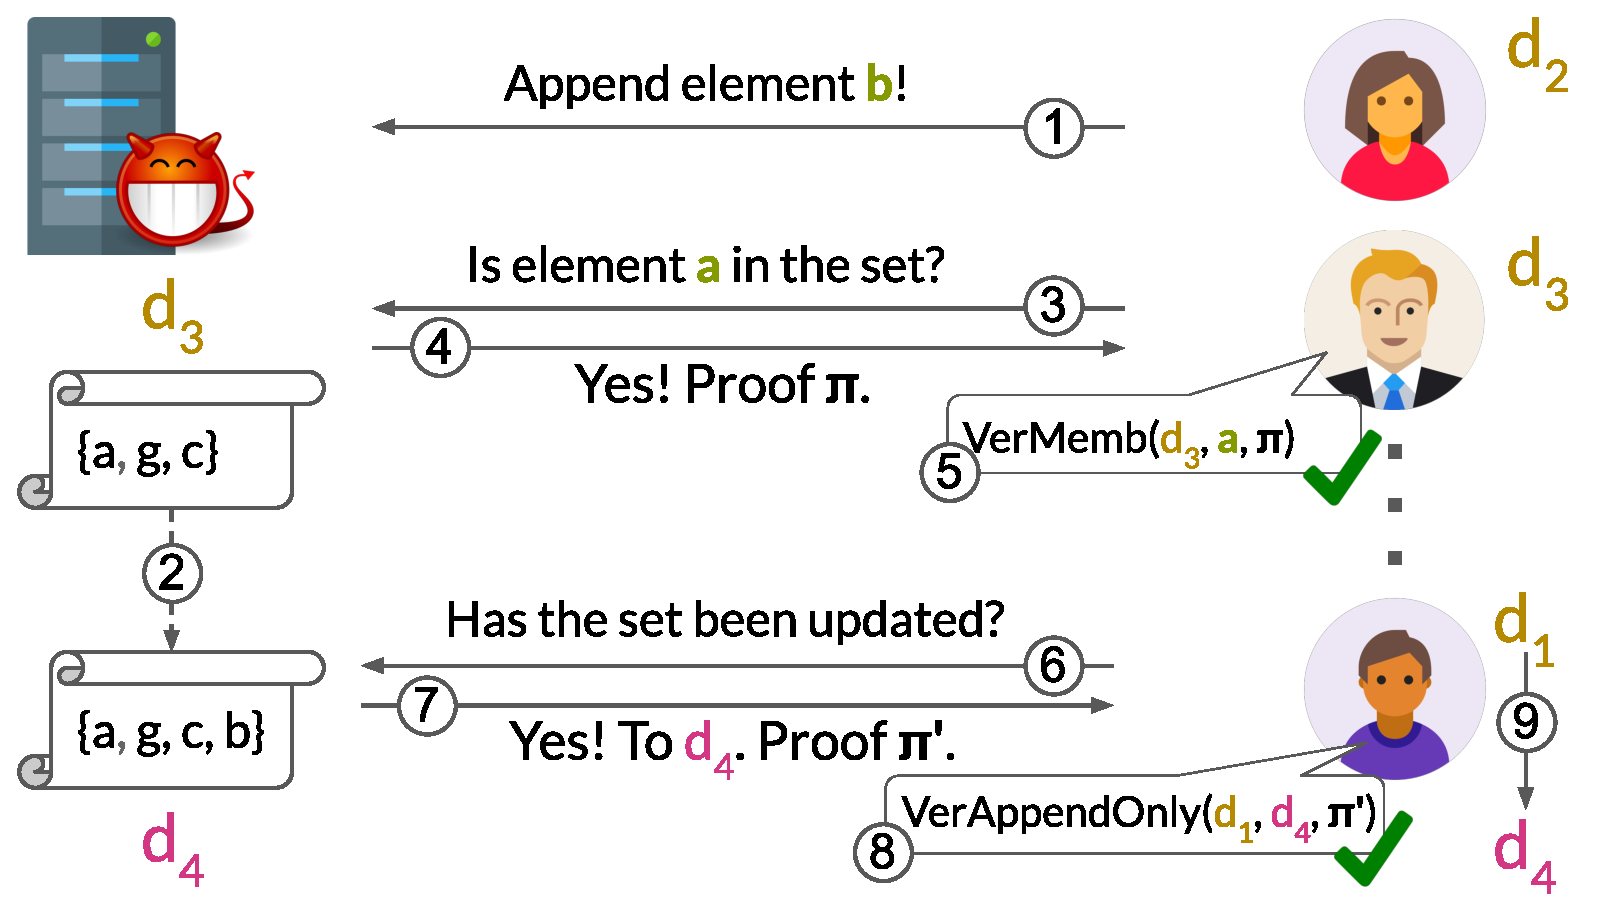
\includegraphics[width=1.0\columnwidth]{figures/model.pdf}
    \vspace{-.5cm}
    \caption{
        Our model: a single malicious \textit{server} manages a \textit{set} and many \textit{clients} query the set.
        Clients will not necessarily have the digest of the latest set.
        The clients can (1) append a new element to the set, (2) query for an element and (3) ask for an updated digest of the set.
    }
    \label{f:model}
    \vspace{-1.5em}
\end{figure}
}

\figModel

\section{Append-only Authenticated Sets}
\label{s:aas}

We begin by introducing a new primitive called an \textit{append-only authenticated set} (AAS).
An AAS can be used for Revocation Transparency (RT) as proposed by Google~\cite{rev-transparency}.
In \cref{s:aad}, we modify our AAS into an \textit{append-only authenticated dictionary} (AAD), which can be used for generalized transparency~\cite{general-transparency}.

\parhead{Overview.}
An AAS is a set of \textit{elements} managed by an \textit{untrusted server} and queried by \textit{clients}.
The server is the sole author of the AAS: it can append elements on its own and/or accept elements from clients.
% e.g., from History Tree paper: "Tamper-evident logs are fundamentally different: An untrusted logger is the sole author of the log and is responsible for both building and signing it.
% This is different from other models where elements might come from a \textit{trusted source} who signs them~\cite{two-party-ad,pads}.
Clients can check membership of elements in the set (see Steps 3-5 in \cref{f:model}).
Clients, also known as \textit{users}, are mutually-distrusting, potentially malicious, and do not have identities (i.e., no authorization or authentication).
Initially, the set starts out empty at \textit{version} zero, with new appends increasing its size and version by one.
Importantly, once an element has been appended to the set, it remains there forever: an adversary cannot remove nor change the element.
After each append, the server signs and publishes a new, small-sized \emph{digest} of the updated set (e.g., Step 2).

Clients periodically update their view of the set by requesting a new digest from the server (e.g., Step 6 and 7).
The new digest could be for an arbitrary version $j > i$, where $i$ is the previous version of the set (not just for $j = i+1$).
Importantly, clients always ensure the set remains \textit{append-only} by verifying an \textit{append-only proof} $\pi_{i,j}$ between the old and new digest (e.g., Step 8).
This way, clients can be certain the malicious server has not removed any elements from the set.
Clients will not necessarily have the latest digest of the set.
Finally, clients securely check if an element $k$ is in the set via a \emph{(non)membership proof} (e.g., Steps 3-5 in \cref{f:model}).

A malicious server can \emph{fork} clients' views~\cite{sundrosdi}, preventing them from seeing each other's appends.
To deal with this, clients maintain a \textit{fork consistent} view~\cite{beyondonethird,sundrosdi} of the set by checking append-only proofs.
As a consequence, if the server ever withholds an append from one client, that client's digest will forever diverge from other clients' digests.
To detect such \textit{forks}, clients can \textit{gossip}~\cite{ct-gossip,cosi,catena,DahlbergPullsVestin2018} with one another about their digests.
This is crucial for security in transparency logs.

This model is the same as in history trees (HTs)~\cite{ht}, assuming only a gossip channel and no trusted third parties.
It also arises in encrypted web applications~\cite{mylar,verena,frientegrity}, Certificate Transparency (CT)~\cite{ct} and software transparency schemes~\cite{at,chainiac}.
Unlike the 2- and 3-party models~\cite{two-party-ad,pads,balloon}, there is no \textit{trusted source} that signs appends in this model.
A trusted source trivially solves the AAS/AAD problem as it can simply vouch for the data structure's append-only property with a digital signature.
Unfortunately, this kind of solution is useless for transparency logs~\cite{ct,ect,coniks}, which lack trusted parties.

%\subsection{Append-only Authenticated Set API}

\parhead{Server-side API.}
The untrusted server implements:
\vspace{.5em}

\api {\setup}$(1^\lambda, \beta) \rightarrow pp, VK$.
Randomized algorithm that returns public parameters $pp$ used by the server and a \textit{verification key} $VK$ used by clients.
Here, $\lambda$ is a security parameter and $\beta$ is an upper-bound on the number of elements $n$ in the set (i.e., $n \le \beta$).

\api {\append}$(pp, \AS_i, d_i, k) \rightarrow \AS_{i+1}, d_{i+1}$.
Deterministic algorithm that appends a new element $k$ to the version $i$ set, creating a new version $i+1$ set.
Succeeds only if the set is not full (i.e., $i + 1 \le \beta$).
Returns the new authenticated set $\AS_{i+1}$ and its digest $d_{i+1}$.

\api $\provememb(pp, \AS_i, k) \rightarrow b, \pi$.
Deterministic algorithm that proves (non)membership for element $k$.
When $k$ is in the set, generates a membership proof $\pi$ and sets $b=1$.
Otherwise, generates a non-membership proof $\pi$ and sets $b=0$.

\api {\proveappendonly}$(pp, \AS_i, \AS_j) \rightarrow \pi_{i, j}$.
Deterministic algorithm that proves $\AS_i \subseteq \AS_j$.
In other words, generates an \textit{append-only proof} $\pi_{i, j}$ that all elements in $\AS_i$ are also present in $\AS_j$.
Importantly, a malicious server who removed elements from $\AS_j$ that were present in $\AS_i$ cannot construct a valid append-only proof.

\parhead{Client-side API.}
Clients implement:
\vspace{.5em}

\api {\vermemb}$(VK, d_i, k, b, \pi) \rightarrow \{T, F\}$.
Deterministic algorithm that verifies proofs returned by $\provememb(\cdot)$ against the digest $d_i$.
When $b=1$, verifies $k$ is in the set via the membership proof $\pi$.
When $b=0$, verifies $k$ is \textit{not} in the set via the non-membership proof $\pi$.
(We formalize security in \cref{s:aas:correctness-and-security}.)

\api {\verappendonly}$(VK, d_i, i, d_j, j, \pi_{i,j}) \rightarrow \{T, F\}$.
Deterministic algorithm that ensures a set remains append-only.
Verifies that $\pi_{i,j}$ correctly proves that the set with digest $d_i$ is a subset of the set with digest $d_j$.
Also, verifies that $d_i$ and $d_j$ are digests of sets at version $i$ and $j$ respectively, enforcing fork consistency.

\parhead{Using the API.}
To use an AAS scheme, first, public parameters need to be computed using a call to $\setup(\cdot)$.
If the AAS scheme is trapdoored, a trusted party or MPC protocol runs $\setup(\cdot)$ and forgets the trapdoor (see \cref{s:discussion}).
Once computed, the parameters can be reused by different servers for different append-only sets.
$\setup(\cdot)$ also returns a \textit{public} verification key $VK$ to all clients.

Then, the server broadcasts the initial digest $d_0$ of the empty set $\AS_0$ to its many clients.
Clients can concurrently start appending elements using $\append(\cdot)$ calls.
If the server is honest, it serializes $\append(\cdot)$ calls.
Eventually, the server returns a new digest $d_i$ to clients along with an append-only proof $\pi_{0,i}$ computed using $\proveappendonly(\cdot)$.
Some clients might be offline but eventually they will receive either $d_i$ or a newer $d_j, j > i$.
Importantly, whenever clients transition from version $i$ to $j$, they check an append-only proof $\pi_{i,j}$ using $\verappendonly(VK, d_i, i, d_j, j, \pi_{i,j})$.

Clients can look up elements in the set.
The server proves (non)\hyp{}membership of an element using $\provememb(\cdot)$.
A client verifies the proof using $\vermemb(\cdot)$ against their digest.
As more elements are added by clients, the server continues to publish a new digest $d_j$ and can prove it is a superset of any previous digest $d_i$ using $\proveappendonly(\cdot)$.

\subsection{AAS Correctness and Security Definitions}
\label{s:aas:correctness-and-security}
We first introduce some helpful notation for our correctness definitions.
Consider an ordered sequence of $n$ appends $(k_i)_{i\in [n]}$.
% NOTE: Can force \newline in inline equations but is there a better way?
% --- begin multiline ---
Let 
$\AS',d' \leftarrow \multiappend(pp, \AS, d, (k_i)_{i\in [n]})$ 
denote a sequence of $\append(\cdot)$ calls arbitrarily interleaved with other $\provememb(\cdot)$ and $\proveappendonly(\cdot)$ calls such that 
$\AS',d'$ $\leftarrow$ $\append(pp,\AS_{n-1}$, $d_{n-1}, k_{n})$,
$\AS_{n-1}, d_{n-1}$ $\leftarrow$ $\append(pp,\AS_{n-2}, d_{n-2}, k_{n-1})$,
$\dots$,
$\AS_{1}, d_1$ $\leftarrow$ $\append(pp,\AS, d, k_{1})$.
% --- end of multiline ---
Finally, let $\AS_0$ denote an empty AAS with empty digest $d_0$.

\begin{definition}[Append-only Authenticated Set]
    \label{d:secure-aas-definition}
    (\setup, \append, \provememb, \proveappendonly, \vermemb, \verappendonly) is a secure append-only authenticated set (AAS) if
    $\exists$ a negligible function $\negl$,
    $\forall$ security parameters $\lambda$,  $\forall$ upper-bounds $\beta=\poly(\lambda)$ and $\forall n \le \beta$ it satisfies the following properties:
\end{definition}

\parhead{Membership correctness.}
\label{s:aas:membership-correctness}
$\forall$ ordered sequences of appends $(k_i)_{i\in[n]}$, for all elements $k$, where $b=1$ if $k\in (k_i)_{i\in[n]}$ and $b=0$ otherwise,
\begin{align*}
\small
\Pr \left[ \begin{array}{c}
(pp,VK) \leftarrow \setup(1^\lambda, \beta),\\
(\AS, d) \leftarrow \multiappend(pp, \AS_0, d_0, (k_i)_{i\in[n]}),\\
(b',\pi) \leftarrow \provememb(pp,\AS, k): \\
{{b=b'}\wedge{\vermemb(VK, d, k, b, \pi) = T}}
\end{array} \right]
\ge 1 - \negl(\lambda)
\end{align*}

\noindent \textit{Observation:}
Note that this definition compares the returned bit $b'$ with the ``ground truth'' in $(k_i)_{i\in[n]}$ and thus provides membership correctness.
Also, it handles non-membership correctness since $b'$ can be zero.
Finally, the definition handles all possible orders of appending elements.

\parhead{Membership security.}
\label{s:aas:membership-security}
$\forall$ adversaries \textsf{A} running in time $\mathsf{poly}(\lambda)$,
\begin{align*}
\small
\Pr \left[ \begin{array}{c}
(pp,VK) \leftarrow \setup(1^\lambda, \beta), \\
(d, k,\pi,\pi') \leftarrow \mathsf{A}(pp, VK)
: \\
{\vermemb(VK,d, k,0,\pi ,) = T} \wedge {} \\
{\vermemb(VK,d, k,1,\pi',) = T}
\end{array} \right] \le \negl(\lambda)
\end{align*}

\noindent \textit{Observation:}
This definition captures the lack of any ``ground truth'' about what was inserted in the set, since there is no trusted source in our model.
Nonetheless, given a fixed digest $d$, our definition prevents \textit{all} equivocation attacks about the membership of an element in the set.
% Note that this definition implies that different sets cannot have the same digest.
% Suppose you have two different sets with the same digest.
% Then membership correctness says you can create proofs for all elements that pass verification.
% Since the sets differ, there exists an element $x$ that is in one set but not the other.
% Yet we will have both membership and non-membership proofs of $x$ that verify w.r.t. the same digest.
% But this breaks membership security. Contradiction.

\parhead{Append-only correctness.}
\label{s:aas:appendonly-correctness}
$\forall m < n,\forall$ sequences of appends $(k_i)_{i\in[n]}$ where $n\ge2$,
\begin{align*}
\small
\Pr \left[ \begin{array}{c}
(pp,VK) \leftarrow \setup(1^\lambda, \beta) \\
(\AS_m, d_m) \leftarrow \multiappend(pp,\AS_0,d_0,(k_i)_{i\in[m]}),\\
(\AS_n, d_n) \leftarrow \multiappend(pp,\AS_m,d_m,(k_i)_{i\in[m+1,n]}),  \\
\pi \leftarrow \proveappendonly(pp,\AS_m, \AS_n):\\
{\verappendonly(VK, d_m, m, d_n, n, \pi) = T}
\end{array} \right] \ge 1 - \negl(\lambda)
\end{align*}

\parhead{Append-only security.}
\label{s:aas:appendonly-security}
$\forall$ adversaries \textsf{A} running in time $\mathsf{poly}(\lambda)$,
\begin{align*}
\small
\Pr \left[ \begin{array}{c}
(pp,VK) \leftarrow \setup(1^\lambda, \beta)\\
(d_i,d_j,i < j,\pi_a, k,\pi,\pi') \leftarrow \mathsf{A}(pp, VK)
: \\
{\verappendonly(VK, d_i, i, d_j, j, \pi_a) = T} \wedge {}\\
{\vermemb(VK, d_i, k, 1, \pi )  = T} \wedge {}\\
{\vermemb(VK, d_j, k, 0, \pi') = T}
\end{array} \right] \le \negl(\lambda)
\end{align*}

\noindent \textit{Observation:}
This definition ensures that elements can only be added to an AAS.

\parhead{Fork consistency.}
\label{s:aas:fork-consistency}
$\forall$ adversaries \textsf{A} running in time $\mathsf{poly}(\lambda)$,
\begin{align*}
\Pr \left[ \begin{array}{c}
(pp,VK) \leftarrow \setup(1^\lambda, \beta)\\
(d_i\ne d_i',d_j,i<j,\pi_i,\pi_i') \leftarrow \mathsf{A}(pp, VK)
: \\
{\verappendonly(VK, d_i , i, d_j, j, \pi_i) = T} \wedge {}\\
{\verappendonly(VK, d_i', i, d_j, j, \pi_i') = T}\\
\end{array} \right] \le \negl(\lambda)
\end{align*}

\noindent \textit{Observation:}
This is our own version of fork consistency that captures what is known in the literature about fork consistency~\cite{ht,beyondonethird}.
Specifically, it allows a server to fork the set at version $i$ by presenting two different digests $d_i$ and $d_i'$ and prevents the server from forging append-only proofs that ``join'' the two forks into some common digest $d_j$ at a later version $j$.
